\documentclass[a4paper,14pt]{extarticle}
\def\source{/home/osabio/tex/templates}
\input{\source/head.tex}
\irodov{3.66}{Электростатика}
\begin{document}

\begin{figure}[H]
    \centering
    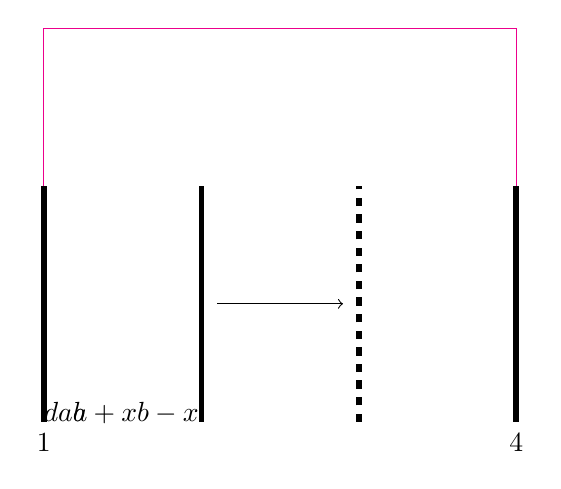
\begin{tikzpicture}
        \draw[line width=2pt] (0,0) node[below] {$1$} -- ++(0,3);
        \draw[line width=2pt] (2,0) -- ++(0,3);
        \draw[->] (2.2,1.5) -- (3.8,1.5);
        \draw[line width=2pt, dashed] (4,0) -- ++(0,3);
        \draw[line width=2pt] (6,0) node[below] {$4$} -- ++(0,3);

        \draw[magenta] (0,3) -- (0,5) -- (6,5) -- (6,3);
        \lineann[-2]{0}{6}{$d$};
        \lineann[-1]{0}{2}{$a$};
        \begin{scope}[xshift=2cm]
	        \lineann[-1]{0}{4}{$b$};
        \end{scope}
        \begin{scope}[yshift=3cm]
	        % \lineann[2]{0}{6}{$d$};
	        \lineann[1]{0}{4}{$a+x$};
	        \begin{scope}[xshift=4cm]
		        \lineann[1]{0}{2}{$b-x$};
	        \end{scope}
        \end{scope}        
    \end{tikzpicture} 
\end{figure}
Рассмотрим суммарное поле слева от пластины в конденсаторе и справа до передвижения. Слева поле конденсатора и пластины вычитаются, справа -- суммируются:
\begin{gather}
	E_L=4\pi\frac{q'}{S}-2\pi\frac{q}{S}=2\pi\frac{2q'-q}{S}\\
	E_R=4\pi\frac{q'}{S}+2\pi\frac{q}{S}=2\pi\frac{2q'+q}{S}
\end{gather}
Аналогично рассмотрим суммарное поле слева от пластины в конденсаторе и справа после передвижения:
\begin{gather}
	E_L'=4\pi\frac{q'+\Delta q'}{S}-2\pi\frac{q}{S}=2\pi\frac{2(q'+\Delta q')-q}{S}\\
	E_R'=4\pi\frac{q'-\Delta q'}{S}+2\pi\frac{q}{S}=2\pi\frac{2(q'-\Delta q')+q}{S}
\end{gather}
Решать будем используя факт замкнутости обкладок конденсатора, т.е. работа по перемещению заряда с одной обкладки на другую равна нулю:
\begin{equation}
	\begin{cases}
		A=0=E_L\cdot a+E_R\cdot (d-a)\\
		A=0=E_L'\cdot (a+x)+E_R'\cdot (d-a-x)\\
	\end{cases}	
\end{equation}
После упрощения:
\begin{equation}
	\begin{cases}
		q'(d-a)+qa=0\\
		(q'-\Delta q')(d-a-x)+q(a+x)=0\\
	\end{cases}	
\end{equation}
Вычтем из второго уравнения системы первое:
\begin{equation}
	(q'-\Delta q')(d-a-x)+qx-q'(d-a)=0
\end{equation}
\begin{equation}
	(q'-\Delta q')(d-a-x)+qx-q'(d-a)=0
\end{equation}

\end{document}